\section{Sensor Technologies for Plant Monitoring}

Every environmental variable, whether soil moisture, temperature, humidity, or light, must be converted into an electrical signal before a controller can process it. The choice of sensor determines not only what can be measured, but also how accurately and how long the system can operate without maintenance. Plant Up! does not target laboratory-grade precision. The engineering goal is stable, repeatable readings that can be compared against defined thresholds and tracked over time.

\subsection{Overview of Common Sensor Types}

\subsubsection*{Soil moisture sensors}

Low-cost soil moisture measurement is typically implemented using resistive or capacitive sensors.

A resistive sensor works by passing a small electric current between two metal probes inserted into the soil. Wet soil conducts electricity better than dry soil, so the measured resistance drops as moisture increases. The principle is straightforward and the hardware is cheap, but there is a significant disadvantage: the metal probes are directly exposed to wet soil, which causes them to corrode over time. As the probes degrade, readings become increasingly unreliable. \cite{chowdhuryCalibration2022}

A capacitive sensor takes a different approach. Instead of measuring how well the soil conducts current, it detects how the surrounding material affects an electric field generated by the sensor. In simple terms, water changes the electrical properties of the soil around the sensor, and this change is what gets measured. The key advantage is structural: the sensing element is embedded inside a coated circuit board, so no metal is directly exposed to the soil. This eliminates the corrosion problem and makes the sensor significantly more durable for long-term use. \cite{seeedCapacitive}

\begin{figure}[H]
    \centering
    \begin{minipage}{0.45\textwidth}
        \centering
        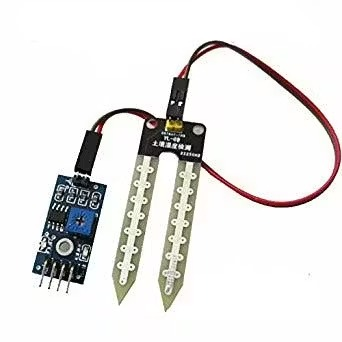
\includegraphics[width=\linewidth]{images/sensor_resistive.png}
        \caption{Resistive Soil Moisture Sensor \cite{hacksterMoistureSensors}}
        \label{fig:sensor_resistive}
    \end{minipage}\hfill
    \begin{minipage}{0.45\textwidth}
        \centering
        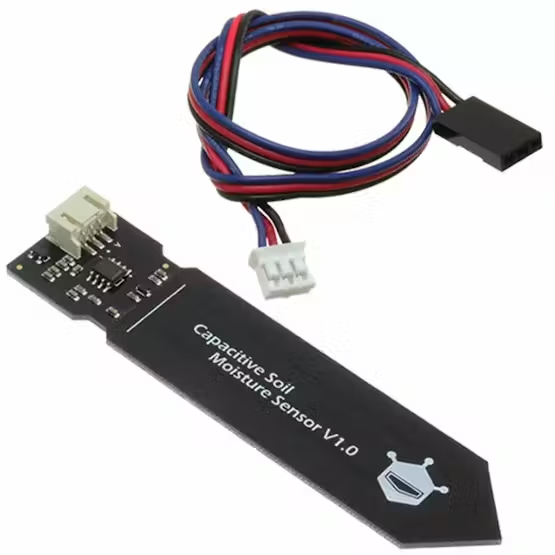
\includegraphics[width=\linewidth]{images/sensor_capacitive.png}
        \caption{Capacitive Soil Moisture Sensor \cite{hacksterMoistureSensors}}
        \label{fig:sensor_capacitive}
    \end{minipage}
\end{figure}

As shown in Figures~\ref{fig:sensor_resistive} and~\ref{fig:sensor_capacitive}, the structural difference is immediately visible. The resistive sensor exposes two metallic forks directly to the soil, while the capacitive sensor uses a sealed PCB surface. This is the core reason why capacitive sensors are generally more suitable for long-term indoor monitoring. \cite{chowdhuryCalibration2022, seeedCapacitive}

\subsubsection*{Temperature and humidity sensors}

Indoor monitoring often uses combined digital sensors such as the BME280. A digital sensor converts the measured value internally and sends a numerical result to the microcontroller, which eliminates the need to interpret raw analog voltages.

The BME280 communicates via I\textsuperscript{2}C, a two-wire protocol that uses one data line and one clock line. Multiple sensors can share the same two wires, which simplifies wiring considerably. For indoor plant monitoring, where detecting trends and crossing thresholds matters more than achieving laboratory-grade accuracy, the BME280 provides sufficient precision. \cite{boschBME280, nxpI2C}

\subsubsection*{Light sensors}

Light intensity can be measured using a photoresistor or a digital lux sensor. A photoresistor changes its resistance depending on brightness. It is simple and inexpensive but mainly useful for relative comparisons within the same setup. A digital lux sensor, by contrast, outputs illuminance directly in calibrated lux values. \cite{bipmPhotometry}

As discussed in the previous chapter, plants respond to light in the PAR range (400--700\,nm), and lux is weighted for human vision rather than plant needs. \cite{nasaPAR2} For basic indoor monitoring, however, lux values are still practical enough to detect whether a plant is receiving adequate or insufficient light.

All three sensor categories, moisture, climate, and light, offer viable solutions for low-cost monitoring. However, selecting the right sensor type is only half the equation. Understanding their practical limitations is equally important, because no sensor delivers perfect data under real-world conditions.

\subsection{Limitations and Typical Error Sources}

\subsubsection*{Non-uniform soil moisture distribution}

Soil inside a pot does not dry evenly. Water moves downward due to gravity, and localized wet zones can persist long after watering.

\begin{figure}[H]
    \centering
    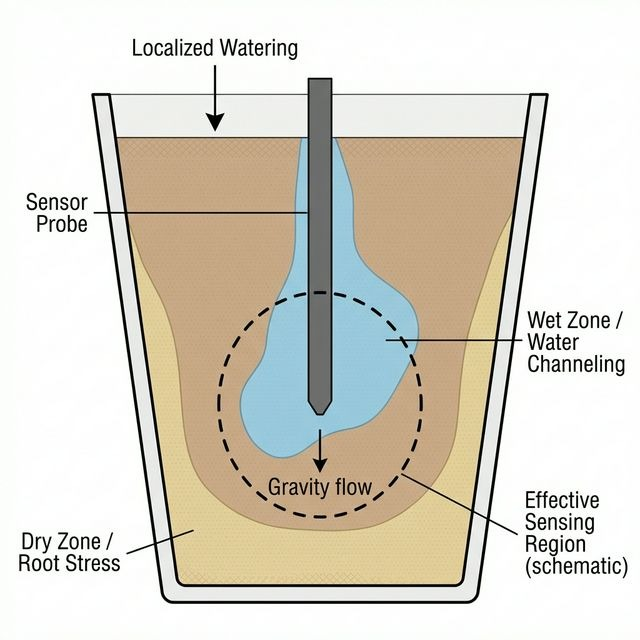
\includegraphics[width=0.6\textwidth]{images/moisture_distortion.png}
    \caption[Measurement distortion caused by non-uniform soil moisture in a plant pot (AI-generated).]{Measurement distortion caused by non-uniform soil moisture in a plant pot. The image illustrates how localized watering can distort sensor readings.}
    \label{fig:moisture_distortion}
\end{figure}

As shown in Figure~\ref{fig:moisture_distortion}, a soil moisture probe only measures a limited region around its body. A single reading may therefore not represent the entire pot. If the sensor happens to sit in a locally wet or dry pocket, threshold-based decisions can become misleading. Consistent sensor placement and insertion depth are therefore essential for reliable monitoring.

\subsubsection*{Sensor drift}

Sensor drift describes a gradual shift in readings over time without any real change in the environment. For resistive sensors, corrosion is the primary driver: as the metal probes degrade, the baseline resistance changes. Capacitive sensors reduce this problem significantly but can still drift due to aging or surface contamination. Periodic validation against a known reference improves long-term reliability. \cite{chowdhuryCalibration2022, seeedCapacitive}

\subsubsection*{Electrical noise and ADC limitations}

Electrical noise refers to unwanted fluctuations in a signal caused by interference or unstable power supply. Analog sensors require an ADC (Analog-to-Digital Converter), which translates a continuous voltage into a discrete digital value. Because the resolution of the ADC is finite, very small moisture changes may not register at all. Hardware quality and basic software filtering, such as averaging multiple readings, therefore directly influence measurement stability.

\subsection{Selection Criteria}

For Plant Up!, a capacitive soil moisture sensor is the preferred choice. It avoids exposed metal electrodes, which eliminates the corrosion failure mode that limits resistive alternatives. This directly improves long-term stability, which is critical for a system intended to run continuously in a home environment. \cite{seeedCapacitive}

Compatibility with the ESP32 microcontroller is another practical constraint. The ESP32 operates at 3.3\,V logic levels, so all selected sensors must support this voltage natively to avoid the need for additional level-shifting circuitry.

In this project, cost and durability outweigh the need for absolute calibration accuracy. The goal is reliable threshold monitoring, not scientific soil analysis. Knowing whether moisture is ``inside the safe corridor'' or ``approaching the danger zone'' matters more than knowing the exact volumetric water content to two decimal places.

Digital sensors such as the BME280 further simplify the hardware design. By communicating over I\textsuperscript{2}C, they reduce analog noise issues and allow multiple sensors to share a single data bus. \cite{boschBME280}

Based on these criteria, the implemented hardware setup of Plant Up! consists of an ESP32 microcontroller, a capacitive soil moisture probe, and a BH1750 digital light sensor. The ESP32 serves as the central processing unit and provides integrated Wi-Fi connectivity as well as 12-bit ADC channels for analog measurements. Its 3.3\,V logic level defines the voltage compatibility requirements for all connected sensors.

The BH1750 light sensor communicates via I\textsuperscript{2}C and directly outputs digital illuminance values in lux within a measurement range of approximately 1 to 65,000\,lux. This avoids additional analog signal conditioning and simplifies integration.

The selected soil moisture probe is designed for 3.3\,V operation and provides an analog voltage proportional to relative substrate moisture. Together, these components form the minimal stable sensing architecture of the system. A detailed component list with supplier information is provided separately.

With the sensor hardware selected and its constraints understood, the next step is to define how these raw electrical signals are collected, transmitted, and processed into usable data. This is where the system moves from simply measuring to actually interpreting.
